\chapter{EMC Effect}	
\section{European Muon Collaboration}\label{sec:EMC}
\paragraph{}The European Muon Collaboration (EMC) performed a deep inelastic measurement with 120-280 GeV muons on iron, hydrogen, and deuteron targets to begin a comprehensive study of ,muon scattering \cite{challenge, Norton}. The EMC used muons in order to reach their goal of achieving interactions at a large $Q^2$ \cite{seelyth}. The EMC studied the per nucleon normalized Fe/D structure function ratio versus the Bjorken scaling variable, $x$. The EMC expectations for this ratio originally was unity for $x$ between 0.05 and 0.7 and would deviate at higher $x$ due to Fermi smearing\cite{CC}. The reasoning for this expectation was the belief that at large magnitude of $Q^2$ the interaction between protons and neutrons would not contribute to the total structure function of the nucleus. This was the understanding because the binding energy of a few MeV would not interferer with the GeV scale of the DIS interaction \cite{Ajth}. The expected structure function for a nucleus could be written as:
\begin{equation}
F_2^A = N F_2^N + ZF_2^P.
\end{equation}
In this quasi-free nucleon picture, the nucleons are used to build up the nuclear structure ($F_2^A$) by summing up the neutron structure function ($F_2^N$) with the proton structure function($F_2^P$) for each nucleon. Their results for their ration comparison of iron and deuterium are shown in Figure \ref{EMCOld}. The $\frac{A}{D}$ structure function ratio showed an unexpected downward slope. This phenomenon was titled the EMC effect. This finding demonstrated to the EMC that their understanding of the nucleus was incorrect. A nucleon's structure function and thereby, the constituent quark distributions are altered by the structure of the nuclear medium. 
\begin{figure}[h]
	\centering
	\caption{ Graph of the ratio of A/D structure functions vs $x$ from the EMC. \cite{CC,EM}.}
	\label{EMCOld}
	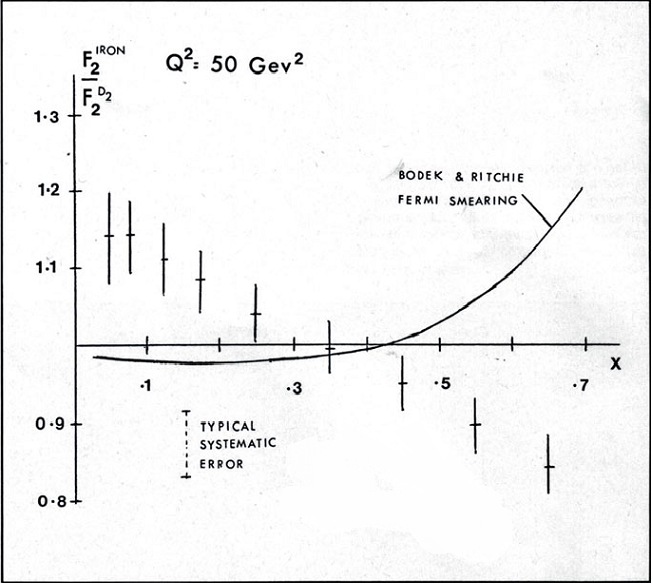
\includegraphics[width=10cm]{EMC.png} 
\end{figure} 
\section{Ratios - Cross Sections and Structure Functions}
\paragraph{}In chapter one we defined the  inelastic cross section in equation \ref{ISCS}.  
\begin{equation}
\label{ISCSch2}
\sigma^A=\frac{4\alpha^2E^{\prime 2}}{Q^4} \bigg\lbrack 2\frac{F_1^A(x)}{M}sin^2\frac{\theta}{2} + \frac{F_2^A(x)}{\nu}cos^2\frac{\theta}{2} \bigg \rbrack.
\end{equation} 
In figure \ref{EMCOld}, the EMC collaboration analyze the ratio of $F_2$ structure functions. The per nucleon cross section of two different nuclei can be reduced to ratio of the $F_2$ structure functions.  
\begin{equation}
\label{rat}
\frac{\sigma_{A_2}}{\sigma_{A_1}} = \frac{F_2^{A_2}}{F_2^{A_1}}
\end{equation}
The reduction of the ratio of two nuclei begin by using the ratio of longitudinal and transverse cross sections as a function of $F_1/F_2$.
\begin{equation}
R=\frac{\sigma_{L}}{\sigma_{T}} =\left(1+\frac{\nu^2}{Q^2} \right)\frac{MF_2}{\nu F_1} -1
\label{Rratio}
\end{equation}
The ratio of two unique per nucleon cross sections is:
\begin{equation}
\label{Aratio}
\frac{\sigma_{A_2}}{\sigma_{A_1}} = \frac{F_2^{A_2}}{F_2^{A_1}} \frac{\left[1+ 2\frac{\nu F_1^{A_2} }{MF_2^{A_2}} tan^2\frac{\theta}{2} \right]}{\left[1+ 2\frac{\nu F_1^{A_1} }{MF_2^{A_1}} tan^2\frac{\theta}{2} \right]}
\end{equation}
Where $A_1$ and $A_2$ denote the different nuclei. Using the definition of $R$ in equation \ref{Aratio}, the per nucleon cross section ratio of $A_1$ and $A_2$ can be simplified to equation \ref{rat} \cite{EM,seelyth}. The simplification of the cross section ratio to the structure function ratio is based on the use of $R$. The longitudinal and transverse cross section ratio has been study extensively for many nuclei. The measurements of $R$ have shown no dependence on the number of nucleons \cite{EM}. 
\paragraph{}The $x$ spectrum of a per nucleon cross section ratio of some nucleus with A nucleons and deuterium also known as an $A/D$ ratio or an EMC ratio is broke into 4 different regions. 
\begin{itemize}
	\item For $x < 0.1$, the shadowing region has an EMC ratio that shows a decline of the nuclear stricture functions. A coupling of the photon to strongly interacting quarks causes this feature \cite{PnN}.
	\item The anti-shadowing region of the $x$ spectrum lies at $0.1 \leq x < 0.3 $. The results of DIS experiments show an EMC ratio slightly larger then unity in this region. This increase is caused by constructive interference among the multi-scattering amplitudes in the nucleus \cite{shadowing}.
	\item $X$ between 0.3 and 0.7 is the EMC effect region. This region will be discussed furtherer in this chapter.
	\item For $X > 0.7$, the EMC ratio grows rapidly above unity.  This region is the Fermi-motion region. The  motion of the nucleons inside a nucleus creates distribution of the nucleons'  momentum. The convolution between the nucleons' structure function and momentum distribution form the nuclear structure function. This causes nuclear structure function of an A $> 2$ nucleus to rise quickly compared to a deuterium nucleus \cite{Ajth,PnN}. 
\end{itemize}
\section{EMC Experiments}
\subsection{EMC at CERN}
\paragraph{} The EMC published results from muon beam experiments in 1981-1983 \cite{EM,EMC_iron,CERN_EMC,EMC_F2d}.  The EMC used data from this group of experiments to form the first EMC ratios, shown in \ref{EMCOld}. The experiments used muon beams of 120 to 280 GeV to extract nuclear and nucleon structure functions from iron, deuterium and Hydrogen targets. The use of multiple indecent beam energies allowed these experiments to have a $Q^2$ for $x$ of 0.05 between 8 and 20 GeV$^2$ and a $Q^2$ for $x$ of 0.65 between 35 and 200 GeV$^2$ \cite{CERN_EMC}. Through out the this run of experiments the EMC used the same apparatus but the experiments were conducted at different times causing a rise in the total uncertainties. After publishing the results for the EMC effect, the EMC conducted another round of experiments for two reasons. First the EMC focused on decreasing the systematic uncertainties that were seen in the first EMC effect analysis. They also want to expand the knowledge of the EMC effect of more nuclei \cite{EMC_ext, Ajth}. This included measuring muon scattering on carbon, copper, and tin \cite{EMC_ext}.

\subsection{BCDMS at CERN}
Th Bologna-CERN-Dubna-Munich-Saclay(BCDMS) collaboration at CERN continued the study of the EMC effect by comparing their measurement of the cross section of nitrogen and iron to deuterium. This experiment used a 40m long iron toroid magnet with 8 modules consisting of scintillators and multiwire proportional chambers \cite{BCDMS}. The data collect from this spectrometer is shown in figure \ref{fig:BCDMS}. The BCDMS collaboration compares their data to the EMC collaboration, demonstrating the consistency of their measurement for the EMC effect for iron \cite{BCDMS,Norton}. 

\begin{figure}[h]
	\centering
	\caption{EMC effect from BCDMS \cite{BCDMS}}
	\label{fig:BCDMS}
	\centering
	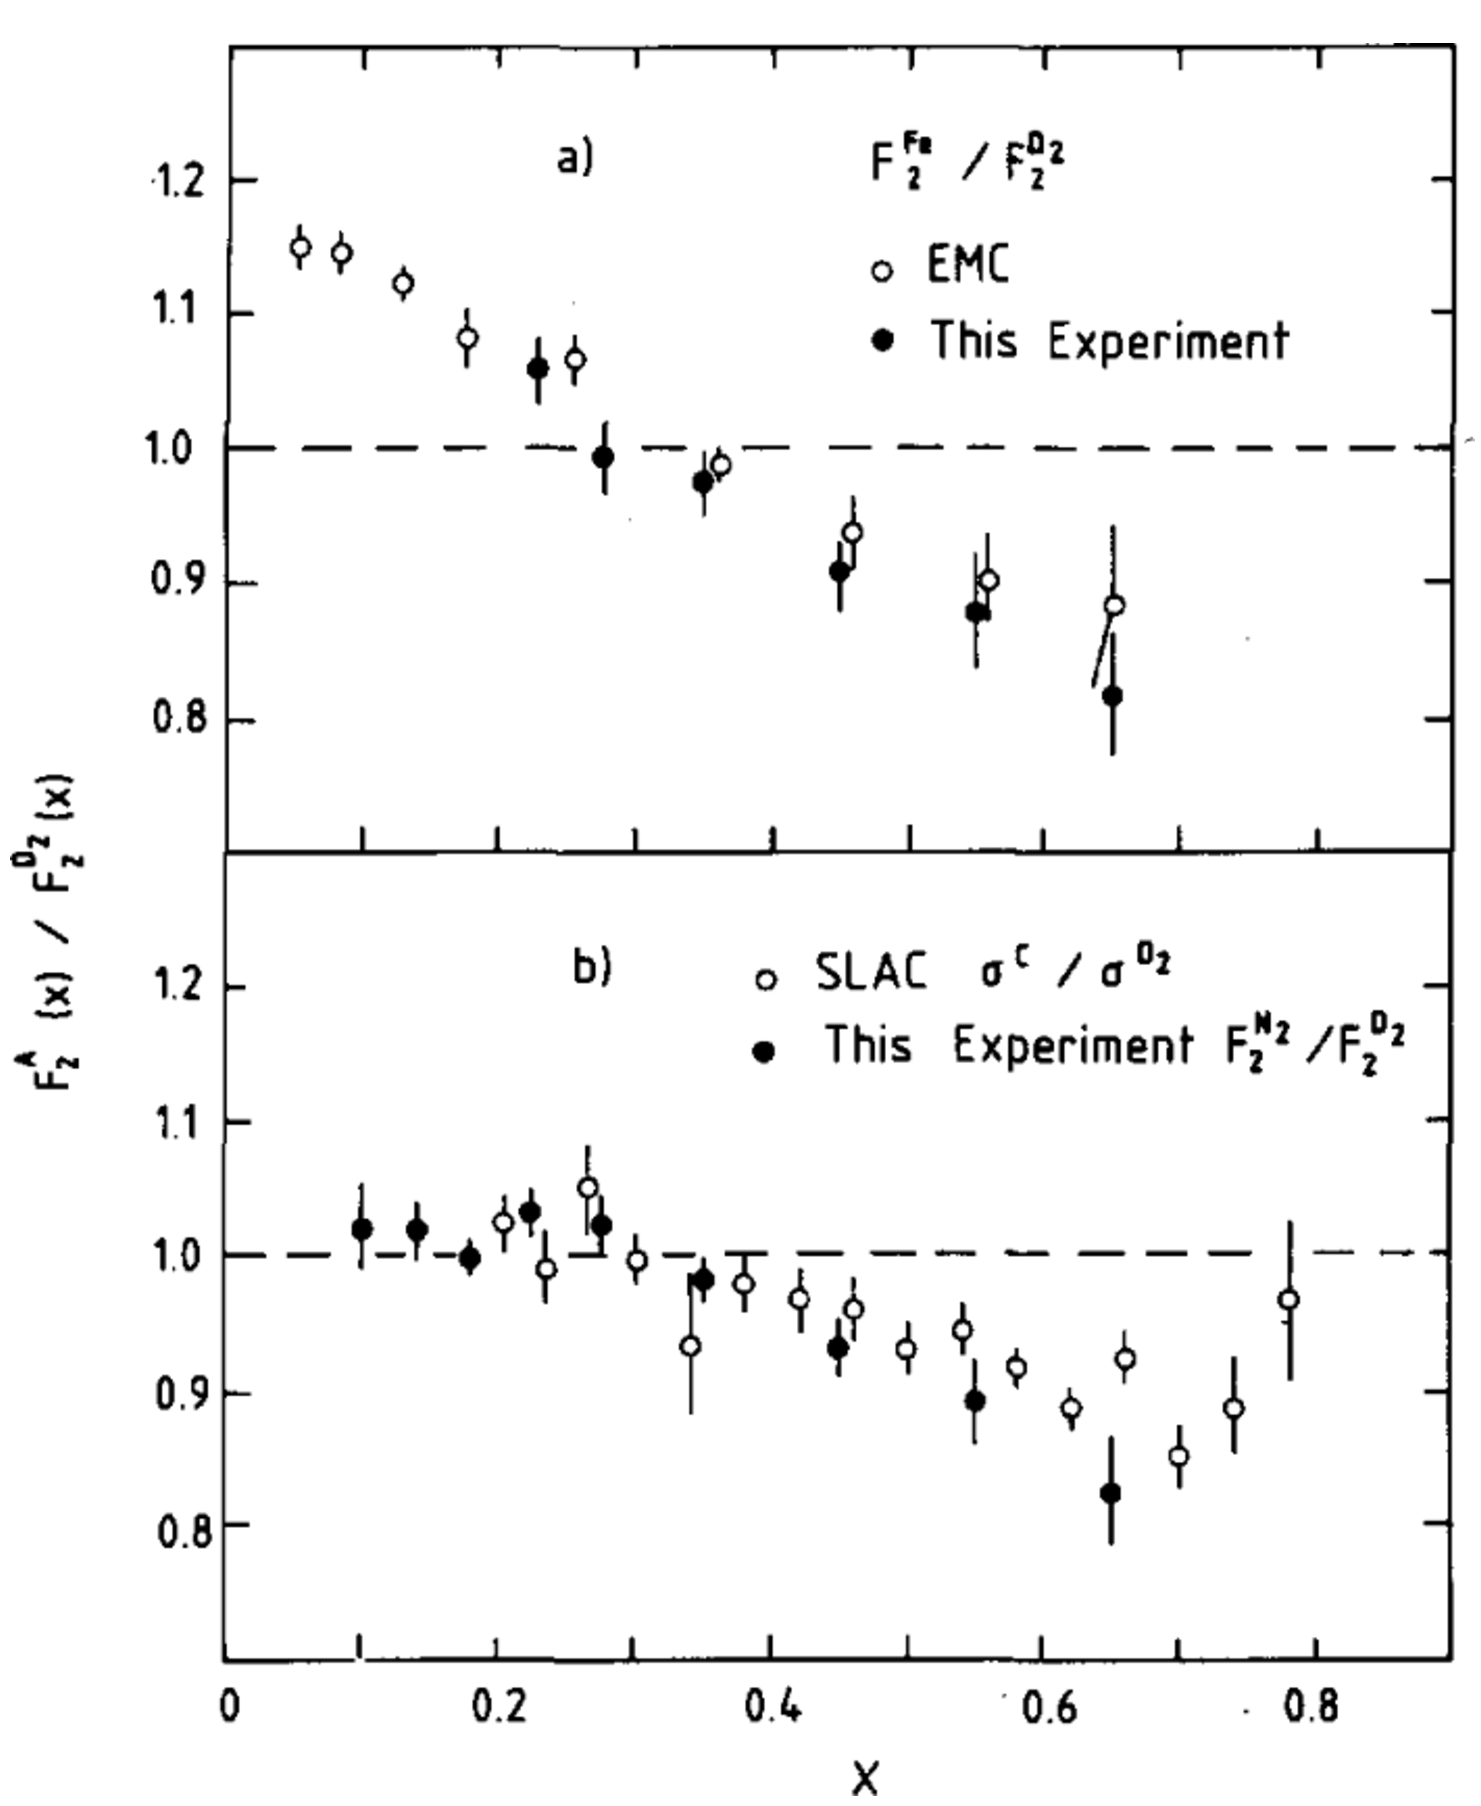
\includegraphics[width=10cm]{BCDMS.pdf}
\end{figure}
\subsection{NMC at CERN}
The New Muon Collaboration(NMC)
\paragraph{}
Scientists at SLAC extracted structure function ratios for many nuclei including; $^4$He, $^9$Be, $^{12}$C, $^{27}$Al, $^{40}$Ca, $^{56}$Fe, $^{108}$Ag, and $^{197}$Au. There were slightly different results for each nucleus. The magnitude of the EMC effect, taken to be the A/D ratio at $x=0.6$, was found to be different for the various nuclei, and roughly scaled with the size or density of the nuclei. The NMC (New Muon collaboration), another group at CERN, gathered precise data in order to construct the inclusive cross section of deuterium and protons. BCDMS collaboration extracted data for N and Fe structure function ratios. Figure \ref{EMC3} shows some of the data from SLAC and BCDMS on the EMC effect for Iron and Cu. Figure \ref{EMC 1} shows this result from a recent JLab EMC measurement, most precise to date. Many models over the years have been able to reproduce the shape of the A/D ratios. These models can contain traditional nuclear physics effects like momentum distribution or pion-charge contributions. Some models also describe the EMC effect through quark momentum distribution or modification of the internal structure \cite{Norton, piler, arri, DF, gomez}. However, no single model has provided a complete picture of the possible underlying physics. Precise data from Jlab's E03-103 experiment has revitalized this research. This experiment focused on precision measurements in light nuclei and added $^{3}$He as a target nucleus. Instead of taking the A/D ratio at a certain $x$-value to be the magnitude of the EMC effect, this analysis looked at the slope instead. This eliminated sensitivity to normalization uncertainties.

\begin{figure}[h]
\centering
\caption{EMC effect from EMC, SLAC, and BCDMS \cite{Norton}}
\label{EMC3}
\centering
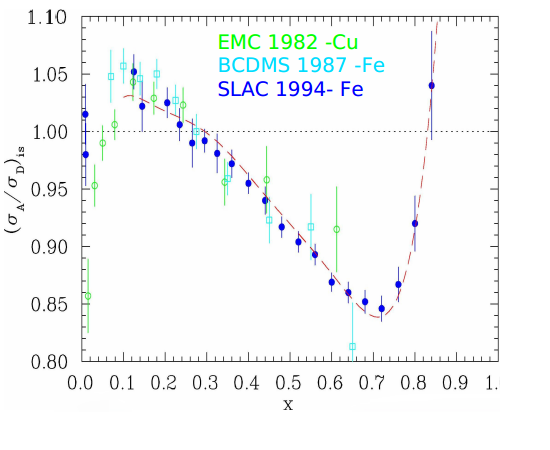
\includegraphics[width=10cm]{EMC3.png}
\end{figure}

\begin{figure}[h]
\centering
 \caption{ Graph of the ratio of A/D structure functions vs $x$ for Carbon \cite{CC}.}
 \label{EMC 1}
 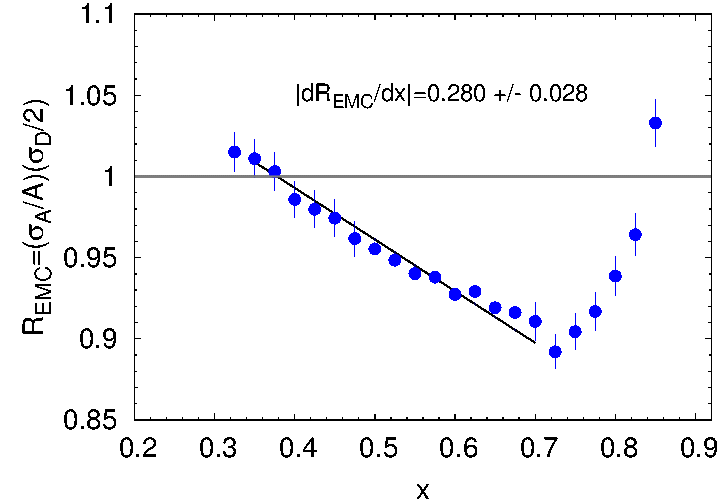
\includegraphics[width=10cm]{EMC1.png} 
 \end{figure} 
 

\paragraph{} In Figure , $^9$Be was found not to follow the previously observed scaling with nuclear density. This result from Jefferson Lab determined that the previous idea of a dependence on A or nuclear density in the EMC effect to be incorrect \cite{seeley}. This result spawned a drive to determine another explanation for the EMC effect and understand what clue the $^9$Be outlier was providing. The structure of this nucleus is made up of two high-density alpha particles and a single neutron \cite{ajppt}. The regions of higher density that are contained in a comparatively large volume may be able to explain why $^9$Be does not follow the expected trend. This suggests that the EMC effect could be a function of local nuclear density \cite{seeley}. 




\section{MARATHON}
Experiment E12-010-102, MARATHON (MeAsurement of the $F2^n$/$F_2^p$,$d$/$u$ RAtios and A=3 EMC Effect in Deep Inelastic Electron Scattering Off the Tritium and Helium MirrOr Nuclei), will use deep inelastic scattering off of the mirror nuclei $^3$H and $^3$He to measure the EMC effect for both $^3$H and $^3$He, to determine the ratio of the neutron to proton inelastic structure functions, and to find the ratio of the down to up quark distributions in the nucleon.

